\documentclass[9pt,aspectratio=169]{beamer}
\mode<presentation>
\usepackage[T1]{fontenc}
\usepackage{color}
\usepackage{graphicx}
\usepackage{natbib}
\usepackage{tikz}
\usetikzlibrary{shapes.geometric}
\usepackage{xmpmulti}
\usepackage{animate}
\usepackage{tcolorbox}
\usepackage{amsmath}
\usepackage{gensymb}
\usepackage{csquotes}
\usepackage{bibentry}
\nobibliography*

\usetheme{Singapore}

\setbeamercolor{block title}{bg=structure!20}
\setbeamercolor{block body}{bg=structure!10}
\setbeamertemplate{blocks}[rounded][shadow]
%\usecolortheme{seahorse}

\usefonttheme{professionalfonts}

\title[Climate Impacts]{Machine learning based evidence and attribution mapping of 100,000 climate impact studies}

\subtitle{Discussion points for resubmission}
%\author{Max Callaghan, Jan Minx, Carl-Friedrich Schleussner, Gerrit Hansen, Quentin Lejeune, Shruti Nath, Emily Theokritoff, Marina Andrijevic, Robert Brecha, Michael Hegarty, Chelsea Jones, Kaylin Lee, Agathe Lucas, Nicole van Maanen, Inga Menke, Peter Pfleiderer, Burcu Yesil }
%\institute[MCC]{
%	
\includegraphics[height=1cm,width=2cm]{images/MCC_Logo_RZ_rgb.jpg} \hspace{5em} 
\includegraphics[height=1cm]{images/climate_analytics.png}
%}

\newif\ifframeinlbf
\frameinlbftrue
\makeatletter
\newcommand\listofframes{\@starttoc{lbf}}
\makeatother

\addtobeamertemplate{frametitle}{}{%
	\ifframeinlbf
	\addcontentsline{lbf}{section}{\protect\makebox[2em][l]{%
			\protect\usebeamercolor[fg]{structure}\insertframenumber\hfill}%
		\insertframetitle\par}%
	\else\fi
}

\newtheorem*{remark}{}

\bibliographystyle{apalike}

\setcounter{secnumdepth}{2}

\begin{document}
	
\begin{frame}
	\titlepage
\end{frame}

\begin{frame}{Discussion points}
\tableofcontents[]
\end{frame}


%%%%%%%%%%%%%%%%%%%%%%%%%%%%%%%%%%%%%%%%%%%%%%%%%%
%% Introduction
\section{Detection and attribution updates}

\begin{frame}{New results from Tom and Shruti}

\begin{columns}
	\begin{column}{0.682\linewidth}
		\begin{figure}
			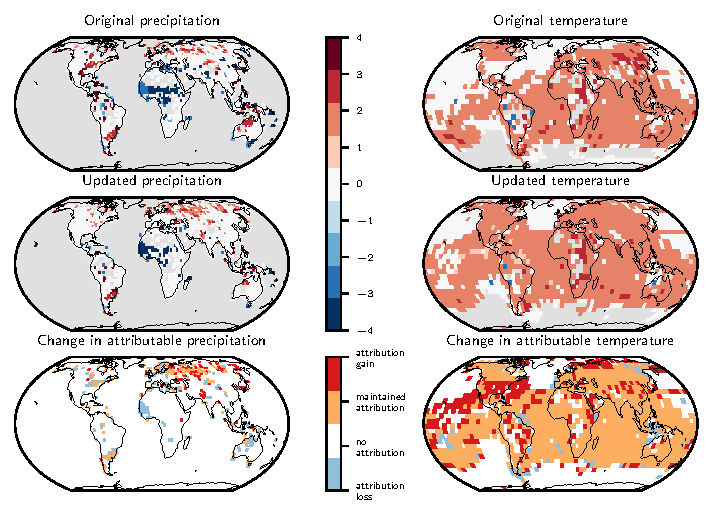
\includegraphics[width=\linewidth]{../plots/attribution_changes.pdf}
		\end{figure}
		
	\end{column}
	\begin{column}{0.318\linewidth}
		\begin{itemize}
			\item Much greater area with attributable temperature trends (particularly N America and oceans)
			\item Some losses of cells with attributable precipitation  (W Africa because of models predicting wrong sign, N America, Australia)
			\item Some additional cells with attributable precipitation in W and NW Asia
		\end{itemize}
	\end{column}
\end{columns}

\end{frame}

\section{Machine learning}

\subsection{Validation procedure}

\begin{frame}{Nested cross-validation}
\begin{columns}
	\begin{column}{0.682\linewidth}
		\begin{figure}
			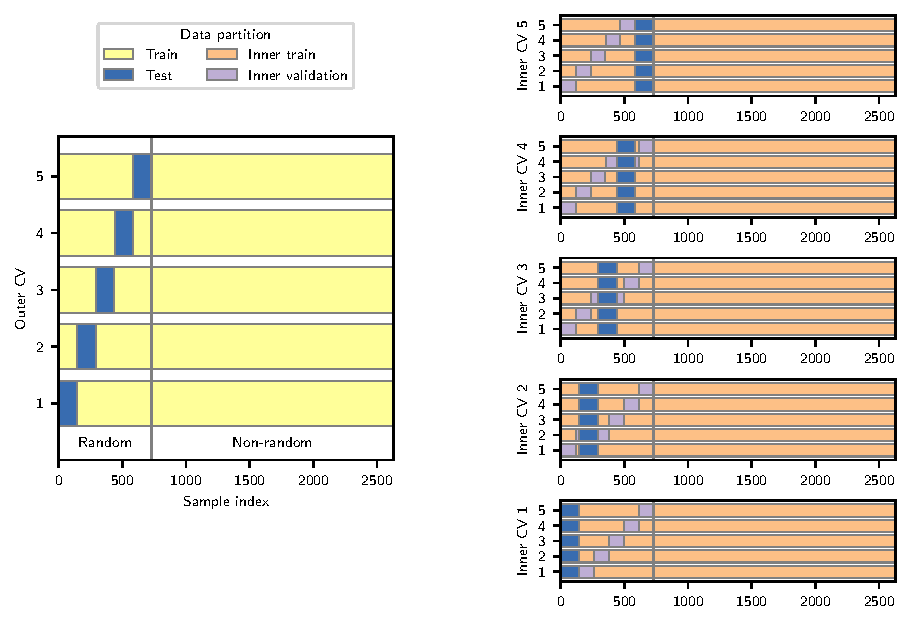
\includegraphics[width=\linewidth]{../figures/si_figure_2.pdf}
		\end{figure}
		
	\end{column}
	\begin{column}{0.318\linewidth}
		\begin{itemize}
			\item We no longer use non-representative samples validation 
			\item Our previous validation procedure (solely cross-validation) was subject to overfitting, and did not systematically explore the parameter space
			\item \textbf{Nested cross-validation} separates the selection of hyperparameters from the validation of model performance 
		\end{itemize}
	\end{column}
\end{columns}
\end{frame}

\subsection{BERT}

\begin{frame}{BERT}
\begin{columns}
	\begin{column}{0.55\linewidth}
		\begin{figure}
			\only<1>{
			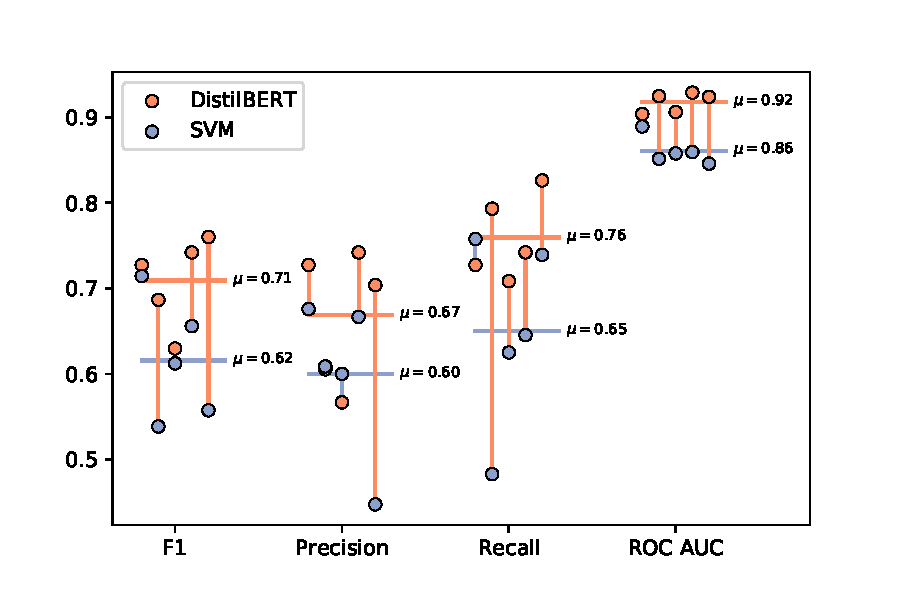
\includegraphics[width=\linewidth]{../figures/SI_figure_3.pdf}
			}
			\only<2>{
				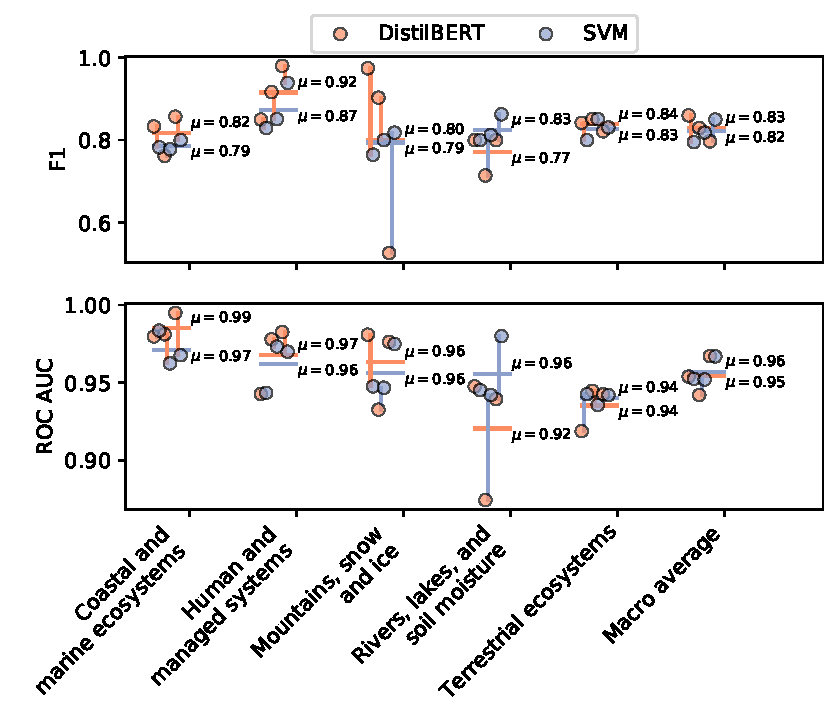
\includegraphics[width=\linewidth]{../figures/SI_figure_4.pdf}
			}
			\only<3>{
				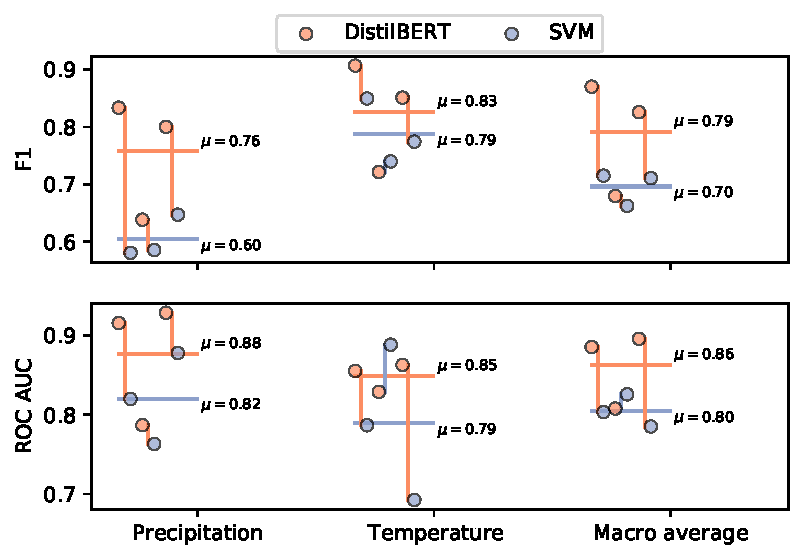
\includegraphics[width=\linewidth]{../figures/SI_figure_5.pdf}
			}
		\end{figure}
	
		How to present these best?
		
	\end{column}
	\begin{column}{0.45\linewidth}
		\begin{itemize}
			\item Our machine learning approach (SVM) was no longer the most cutting edge 
			\item BERT (Bidirectional Encoder Representations from Transformers) type models have in the last couple of years surpassed many benchmarks in NLP tasks.
			\item BERT are large language models trained on large corpora and can be fine-tuned to perform specific classification tasks
			\item DistilBERT (a smaller and faster version of BERT) outperforms SVM
			\item We have poor performance in mountains, snow and ice due to very few examples in the random sample
		\end{itemize}
	\end{column}
\end{columns}
\end{frame}

\section{Explanation and responses}

\subsection{Clarity of process}

\begin{frame}{Clarity of process}

\begin{columns}
	\begin{column}{0.4\linewidth}
		\begin{figure}
			\only<1>{
				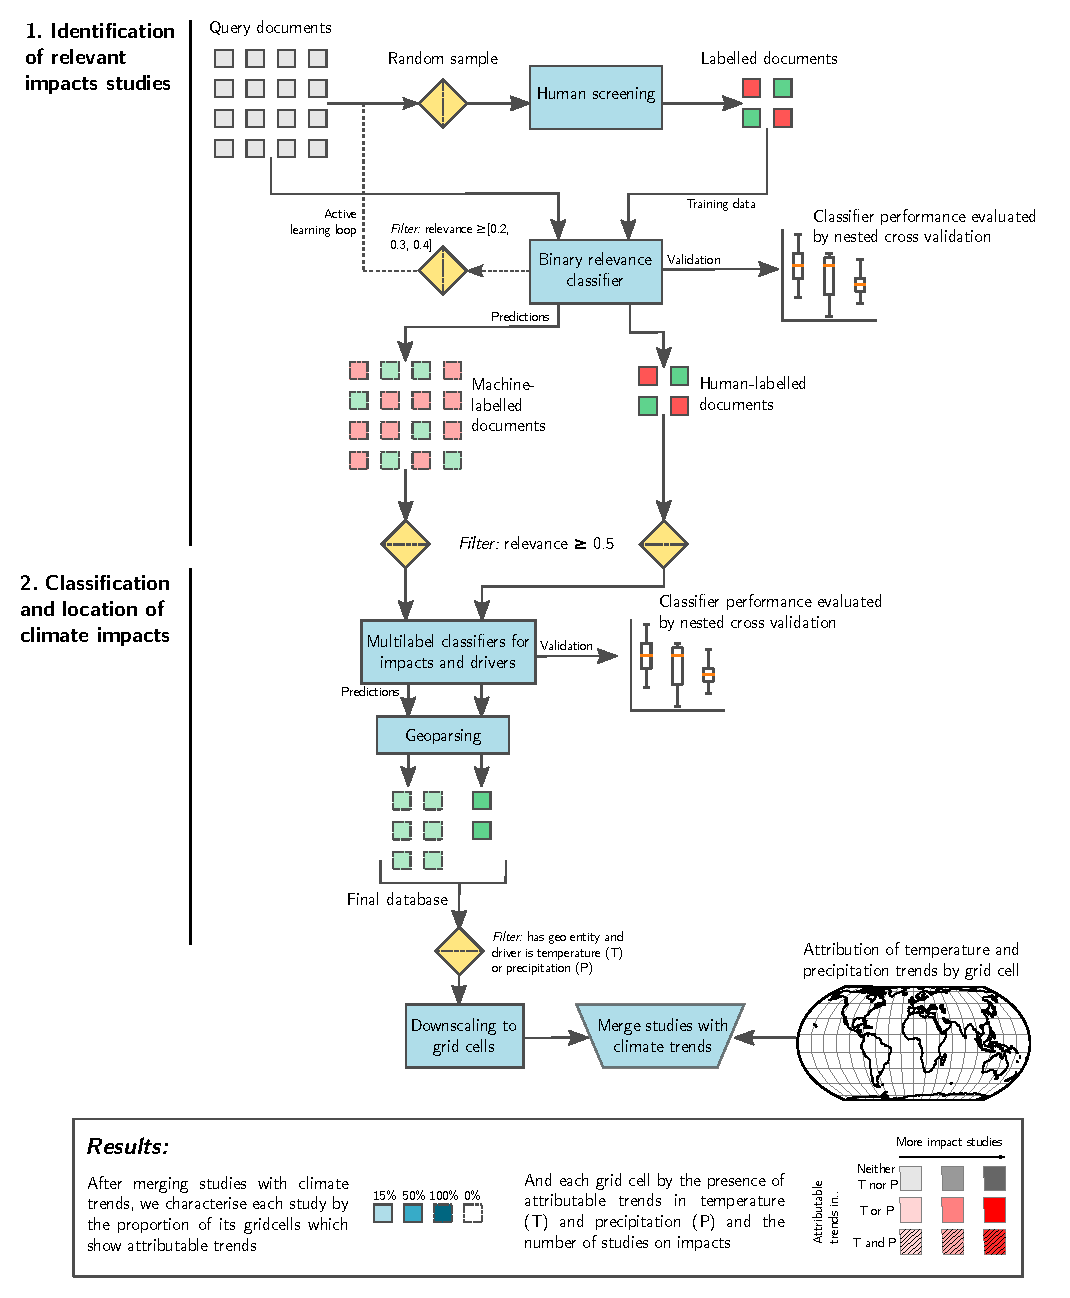
\includegraphics[width=\linewidth]{../figures/process.pdf}
			}
		\end{figure}
		
	\end{column}
	\begin{column}{0.6\linewidth}
		\begin{itemize}
			\item We have a detailed diagram better describing the process
			\item The methods section is significantly rewritten 
		\end{itemize}
	\end{column}
\end{columns}
\end{frame}

\subsection{Abstracts}

\begin{frame}{Abstracts}



	A major sticking point was the use of abstracts and the question of whether this biases our results
	
	\medskip
	\hrule
	\medskip
		

		We respond that
		\begin{itemize}
			\item Abstracts contain the best summary of the topic of a document
			\item Within full texts you have many different types of texts, including reference to other results, which may increase the risk of false positives.
			\item Further, we simplify the information we want to extract from abstracts to 
			\begin{itemize}
				\item Does the article present evidence on climate impacts \textit{broadly defined}?
				\item What \textit{broad} class of impacts does it describe?
				\item Are impacts driven by temperature or precipitation or other variables?
			\end{itemize}
			We no longer distinguish between the type of evidence provided (trends or variability) as it could be argued that abstracts are insufficient to answer this fully.

		\end{itemize}
			In summary, we may miss some documents which present evidence of climate impacts but do not discuss this in the abstract, but in doing so we avoid the (in our opinion likely more common) class of documents where impacts may be discussed in full texts but this is not the focus of the study.


\end{frame}

\section{Updated results}

\subsection{Figure 1}

\begin{frame}{Figure 1}
\begin{columns}
	\begin{column}{0.682\linewidth}
		\begin{figure}
			\only<1>{\includegraphics[width=\linewidth]{../figures/figure_1.pdf}}
			\only<2>{\includegraphics[width=\linewidth]{../old_figures/figure_1.pdf}}
		\end{figure}
		
	\end{column}
	\begin{column}{0.318\linewidth}
		\begin{itemize}
			\item The total number of predicted included results is larger (with more variation)
			\begin{itemize}
				\item Previous model was optimized for marginal decisions and was overly conservative
			\end{itemize}
		 	\item Qualitatively results remain similar
			\item Evidence type is removed
		\end{itemize}
	\end{column}
\end{columns}
\end{frame}

\subsection{Figure 2}

\begin{frame}{Figure 2}
\begin{columns}
	\begin{column}{0.682\linewidth}
		\begin{figure}
			\only<1>{
			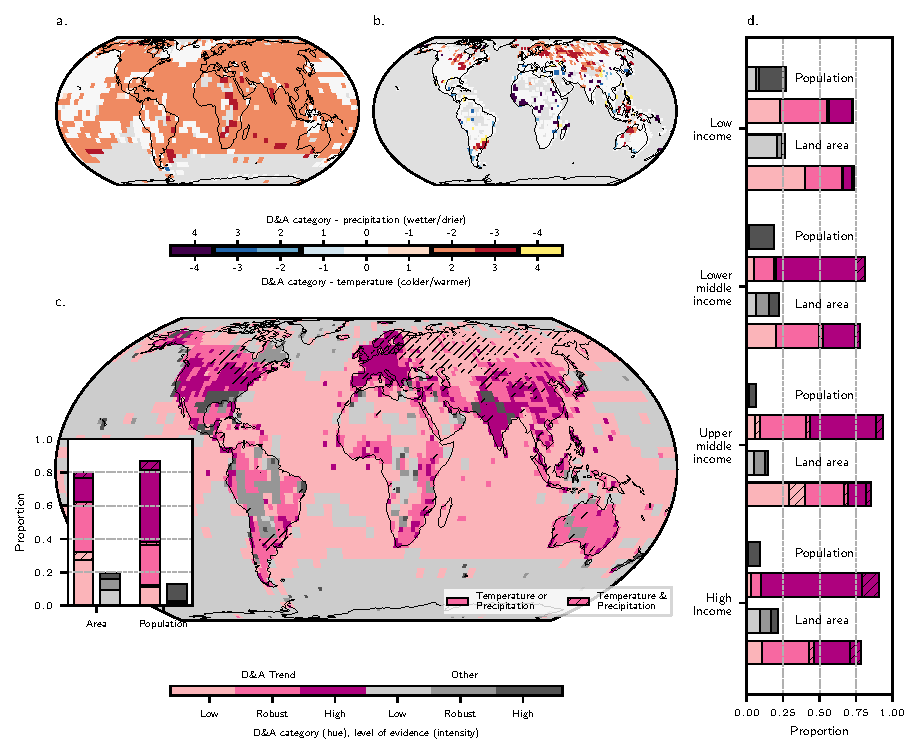
\includegraphics[width=\linewidth]{../figures/figure_2.pdf}
		}
			\only<2>{
	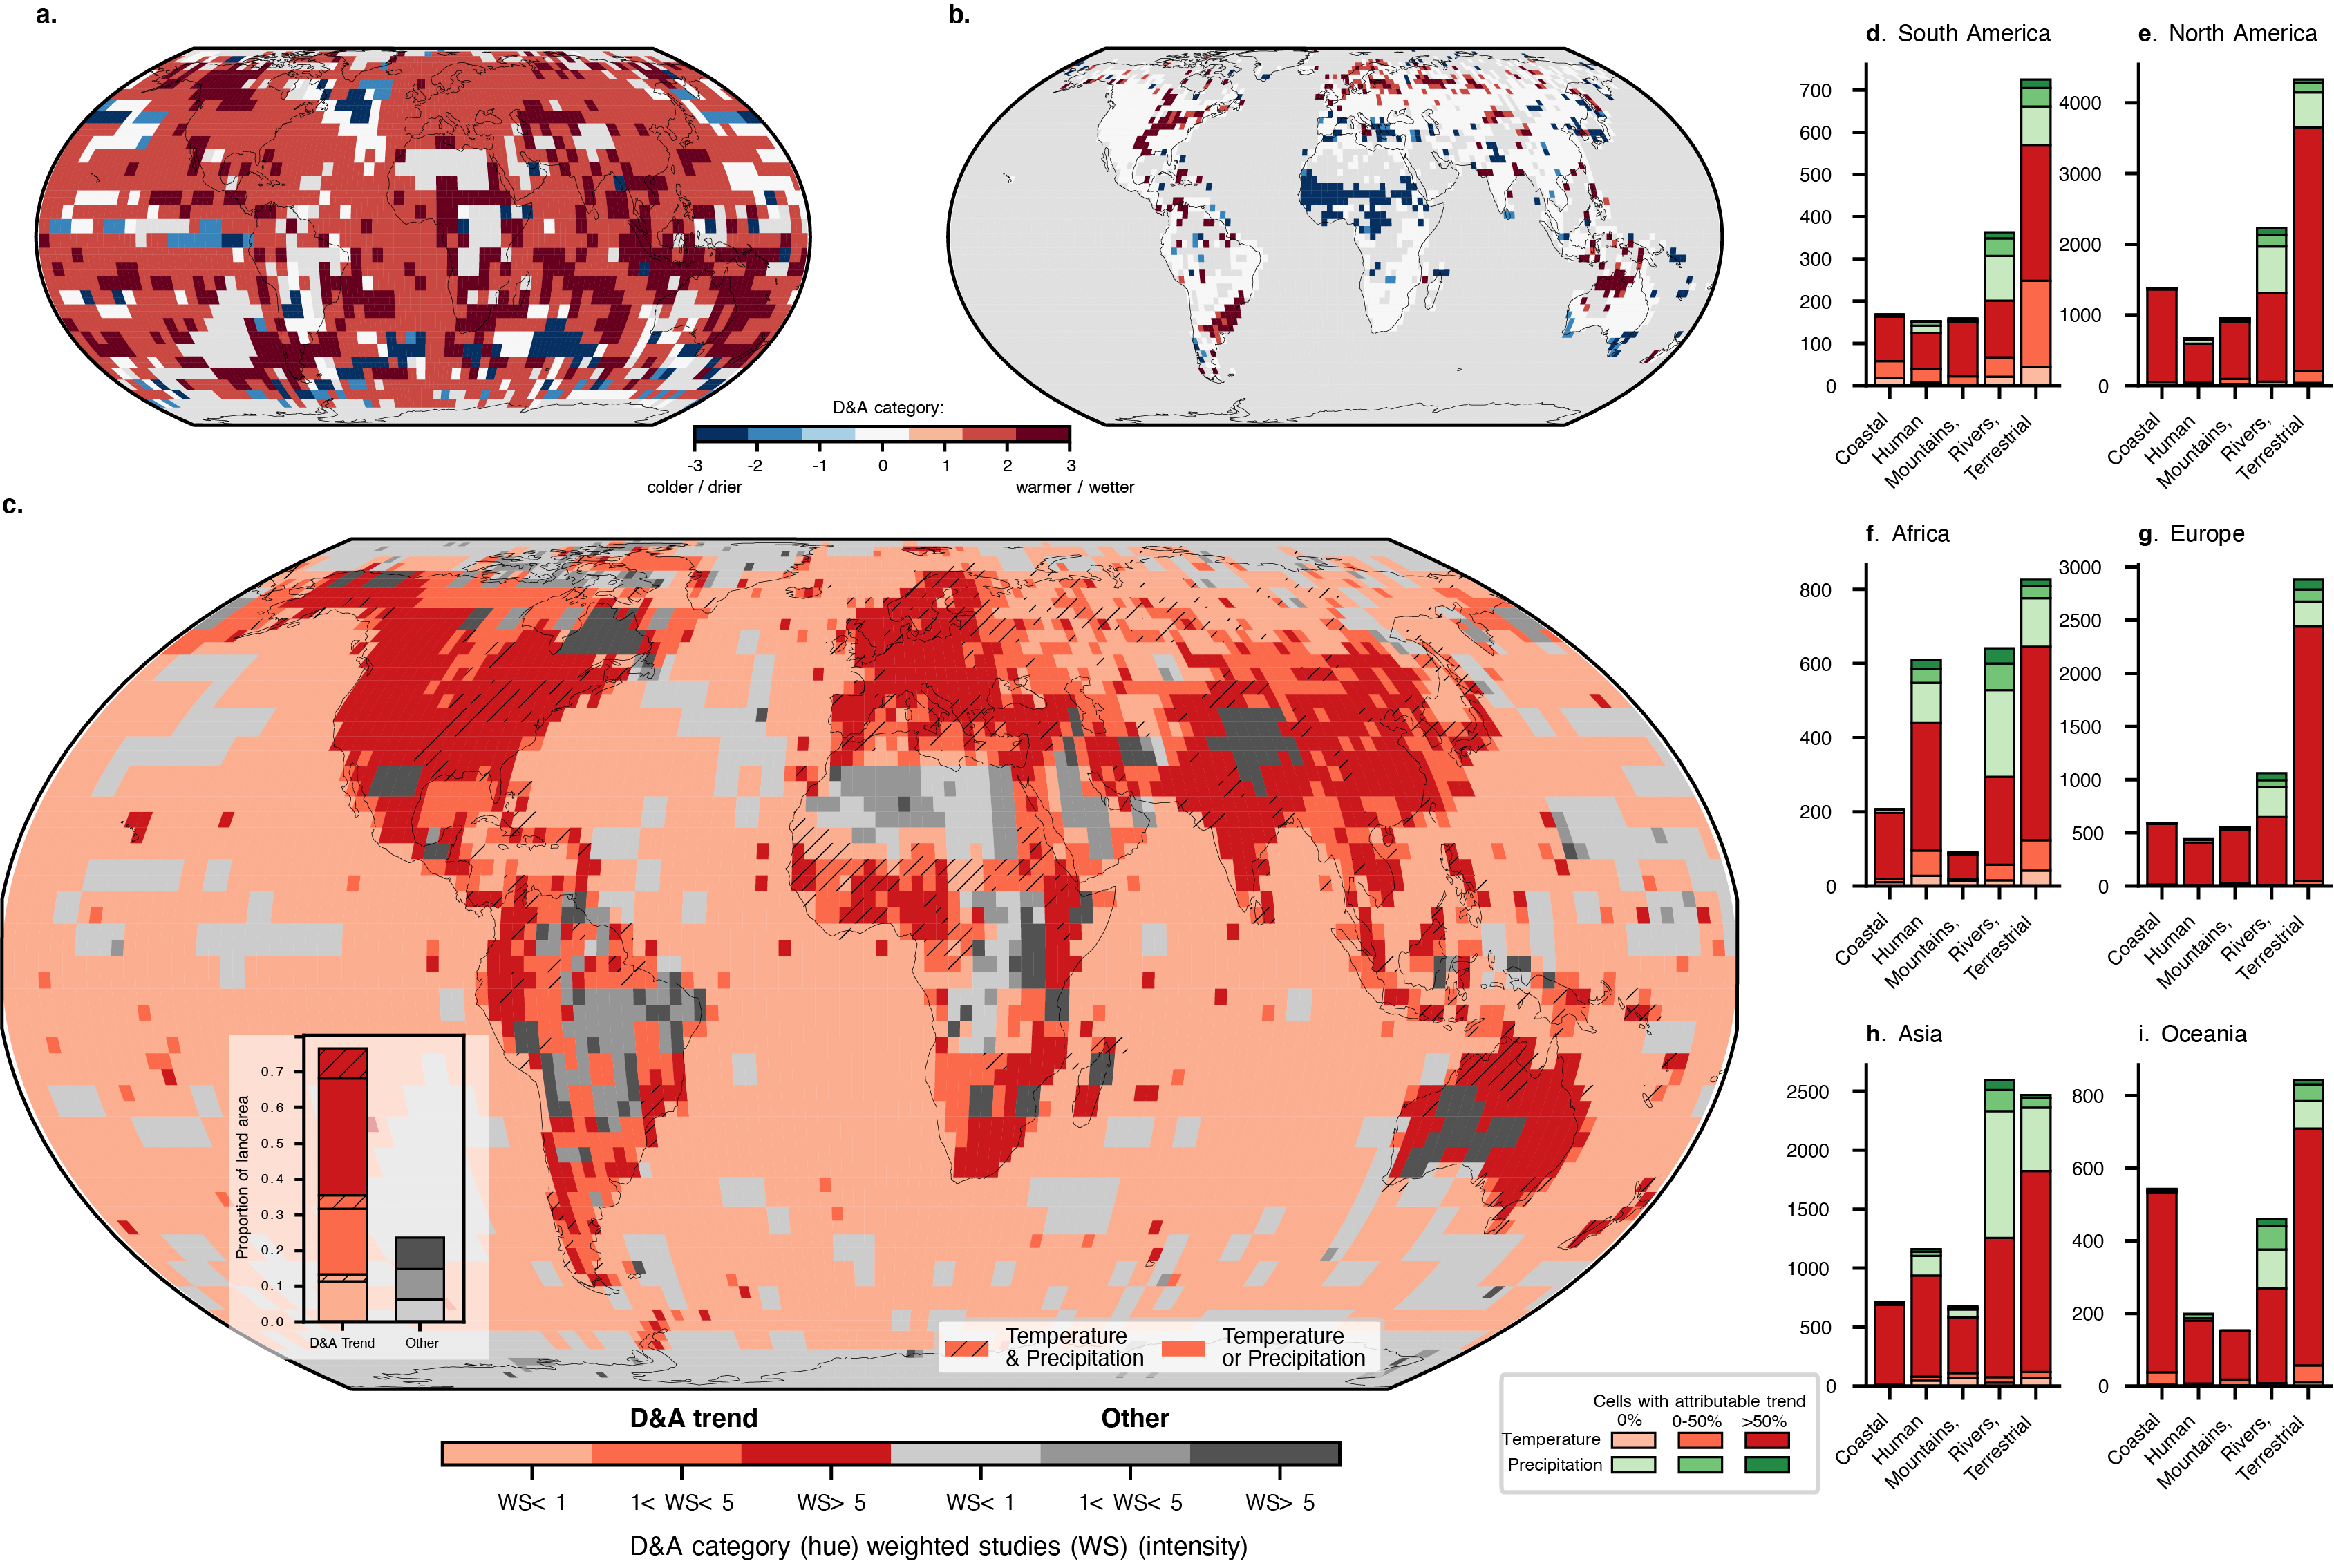
\includegraphics[width=\linewidth]{../old_figures/figure_2_CFS_10_28.png}
}	
		\end{figure}
		
	\end{column}
	\begin{column}{0.318\linewidth}
		\begin{itemize}
			\item Qualitative results are similar
			\item We reset thresholds (now we are including more evidence) to maintain distinction between qualitatively \textbf{lots} and \textbf{little} evidence
			\item Fewer attributable studies for precipitation
		\end{itemize}
	\end{column}
\end{columns}
\end{frame}


\subsection{Figure 3}

\begin{frame}{Figure 3}
\begin{columns}
	\begin{column}{0.5\linewidth}
		\begin{figure}
			\only<1>{
			\includegraphics[width=\linewidth]{../figures/figure_3.pdf}
		}
				\only<2>{
		\includegraphics[width=\linewidth]{../old_figures/figure_3.pdf}
	}
		\end{figure}
		
	\end{column}
	\begin{column}{0.5\linewidth}
		\begin{itemize}
			\item Qualitative results are similar
		\end{itemize}
	\end{column}
\end{columns}
\end{frame}

\section{Next steps}



\begin{frame}{Next steps}
	\begin{itemize}
		
	\item \textbf{Main text}: \url{https://docs.google.com/document/d/17NY4TB0yHsR5TsoTGiRUT6OkigT0LGEjTnN0Bb9UsiI/edit} major updates complete, and feedback from Tom mostly incorporated. 
	\item \textbf{Methods and extended figures}: \url{https://docs.google.com/document/d/1mE3BD8WTQSNSPVtLYHHMVNqryctc8vypDvD5d8WBi30/edit} major updates complete. 
	\item \textbf{Response to reviewers}: \url{https://docs.google.com/document/d/16DSrxjI3MbZVXX-E35RQYdwVzDjsWxPzF0W7zRWv0rM/edit?usp=sharing} needs work in parallel with final close edits to main text. 
	
	\end{itemize}

\end{frame}

\end{document}